
\input preamble.tex
\vskip 5pt

\vskip 5pt
\begin{center}
	\huge
	\textbf{Læringsoppdrag digitale målesystemer - Stasjon 15}
	\normalsize
\vskip 5pt 
\end{center}

$$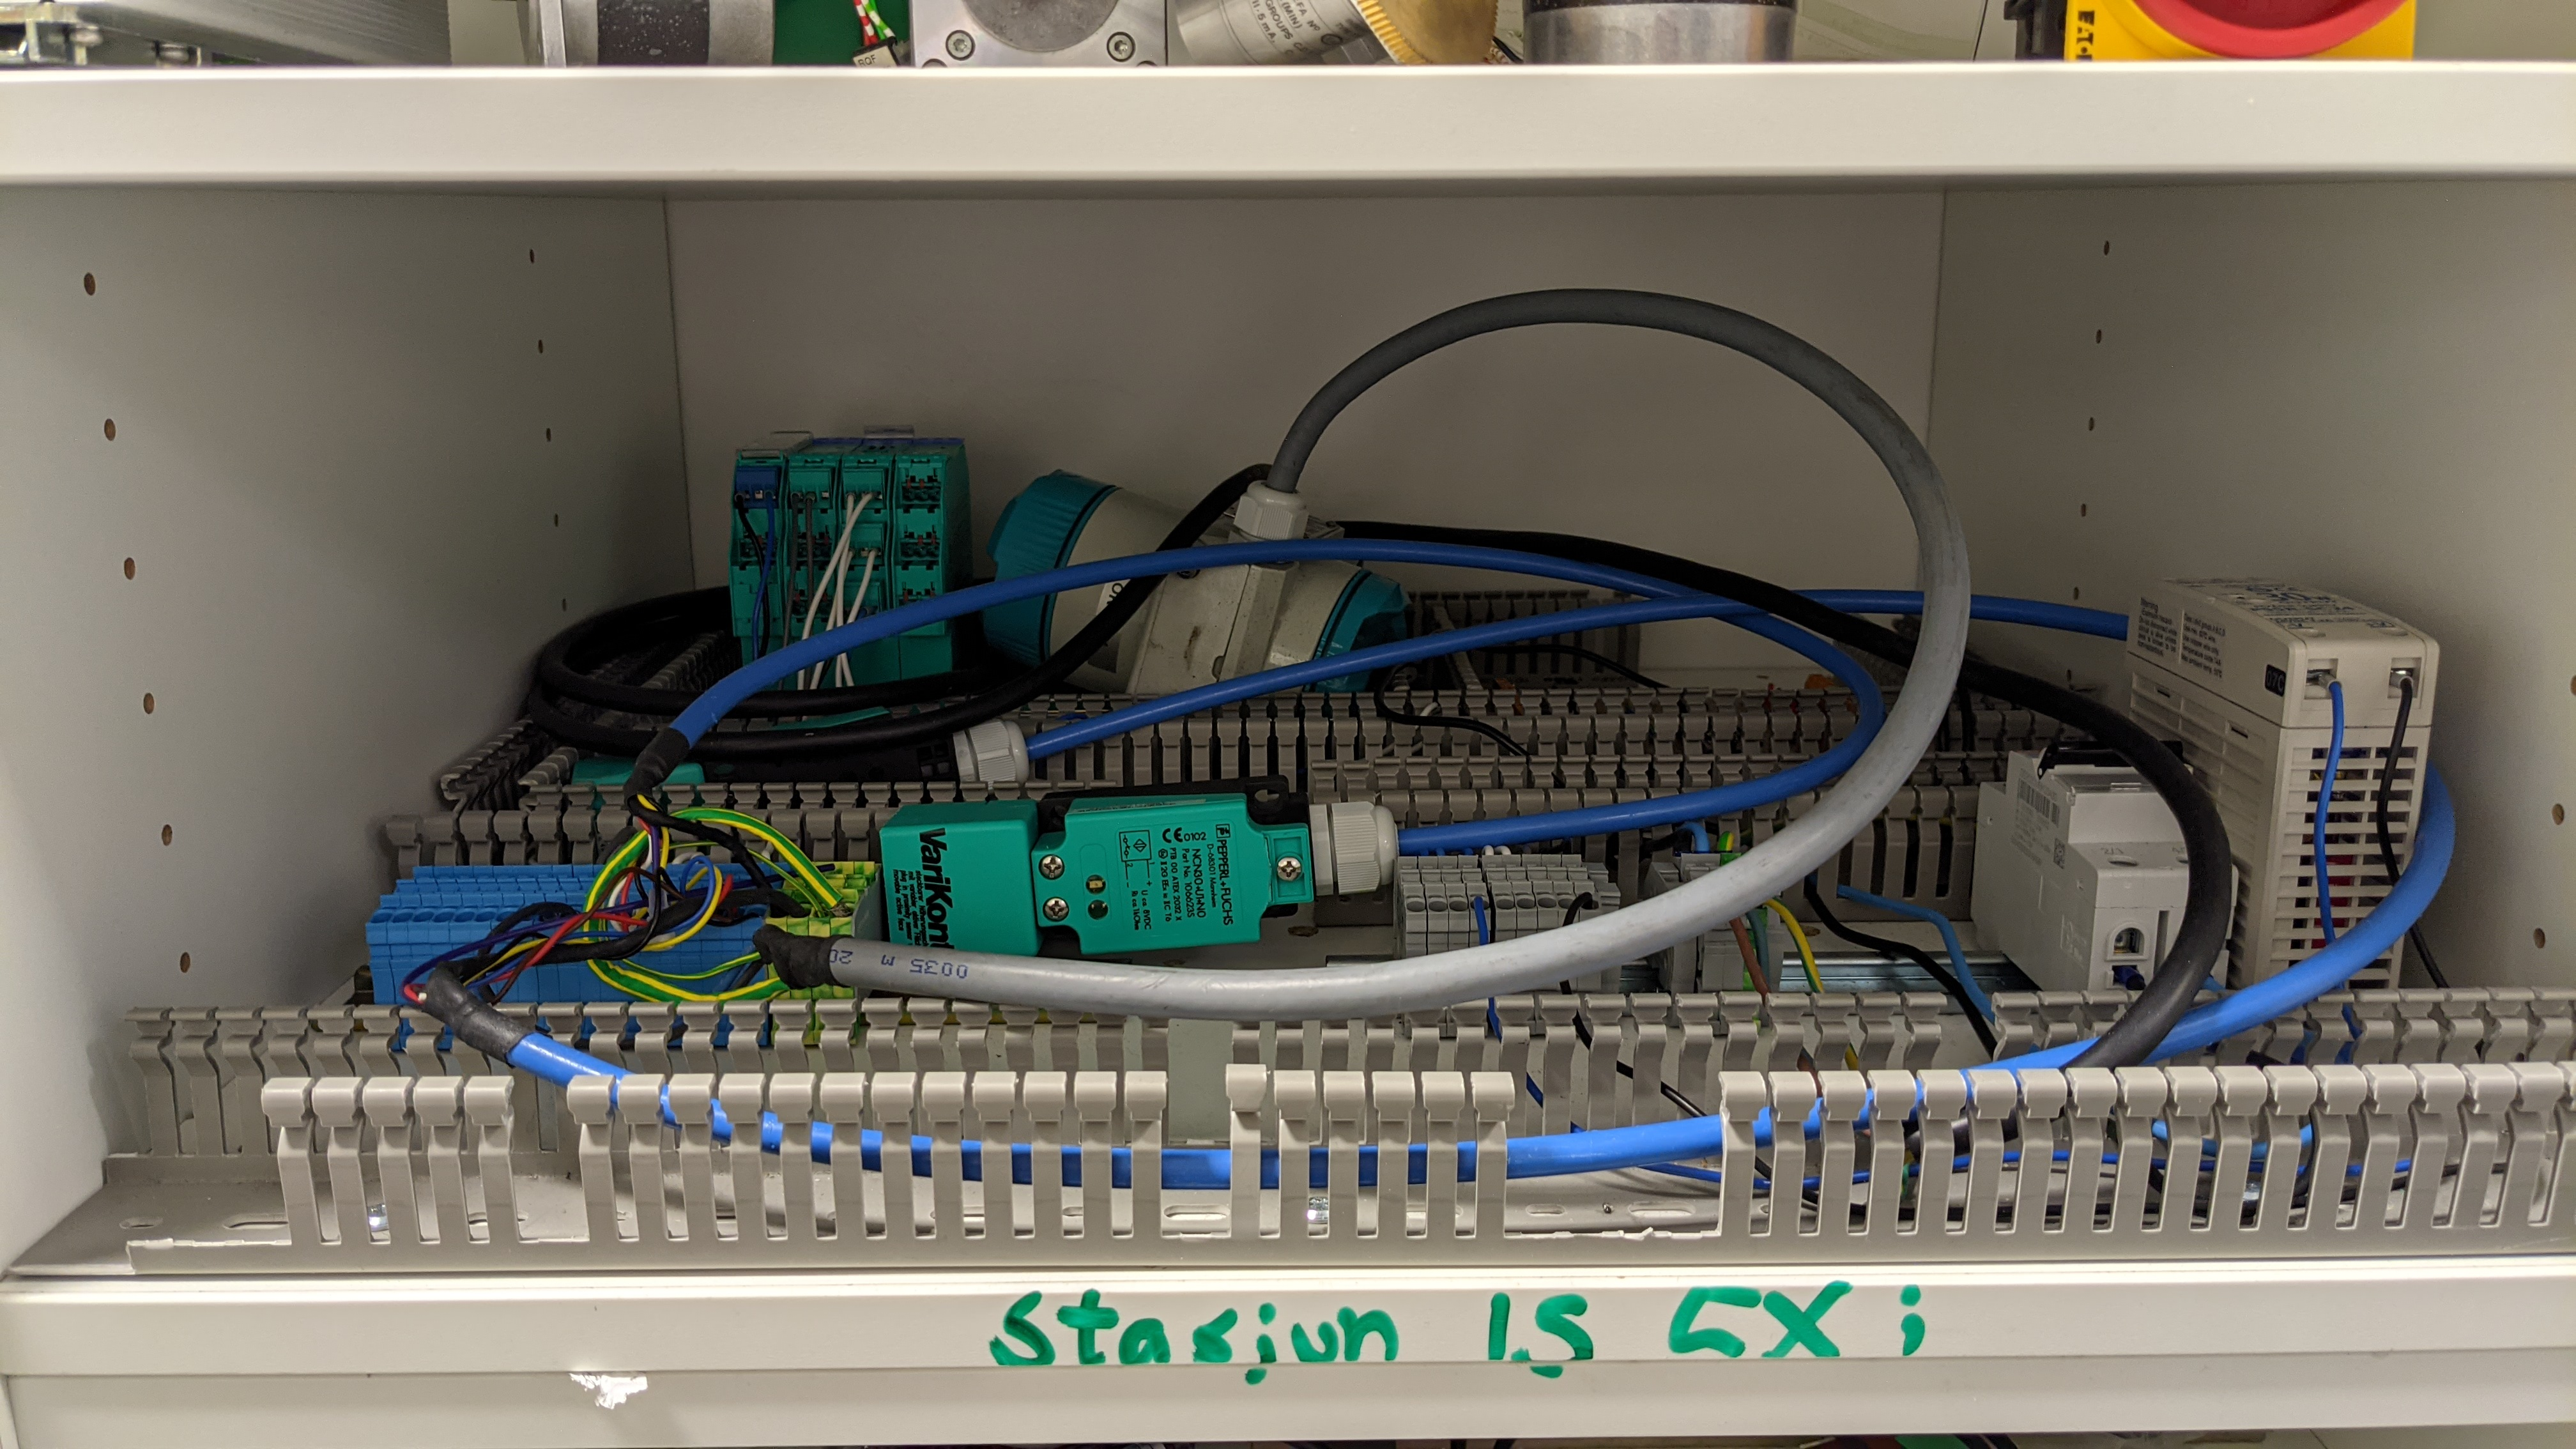
\includegraphics[width=13cm]{./stasjon15x01.jpg}$$\\

\vskip 1cm
Dette læringsoppdraget består av følgende:

\begin{itemize}[noitemsep]
	\item Oppgavesett Temperaturregulering
	\item Arbeidsoppdrag digitale målesystemer 
\end{itemize}


 
\vskip 5pt 

Du kan jobbe parallelt med alle oppgavene. 

\vskip 5pt 
\textbf{Bakgrunnsteori}
 I filen \href {https://autofaget.no/pdfs/afgv.pdf}{afgv.pdf} er følgende kapittler til hjelp for dette læringsoppdraget:
 \begin{itemize}[noitemsep]
	 \item Discrete process measurement
 \end{itemize}

 \vskip 5pt 
\href{https://www.eaton.com/ecm/groups/public/@pub/@electrical/documents/content/pct_1549250.pdf}{The Basics of Limit Switches - Eaton guide til endebrytere}
\newpage
\textbf{Arbeidsoppdrag i digitale målesystemer}

\vskip 1cm

\textbf{Introduksjon}

I denne oppgaven skal du koble opp og teste ulike digitale målesystemer



\begin{enumerate}
\item Mekanisk endebryter med rulle
\item Mekanisk endebryter med fjær
\item Mekanisk endebryter med aksling....
\item kapasitiv nærhetssensor 
\item induktiv nærhetssensor
\item Photo sensor 
\end{enumerate}


$$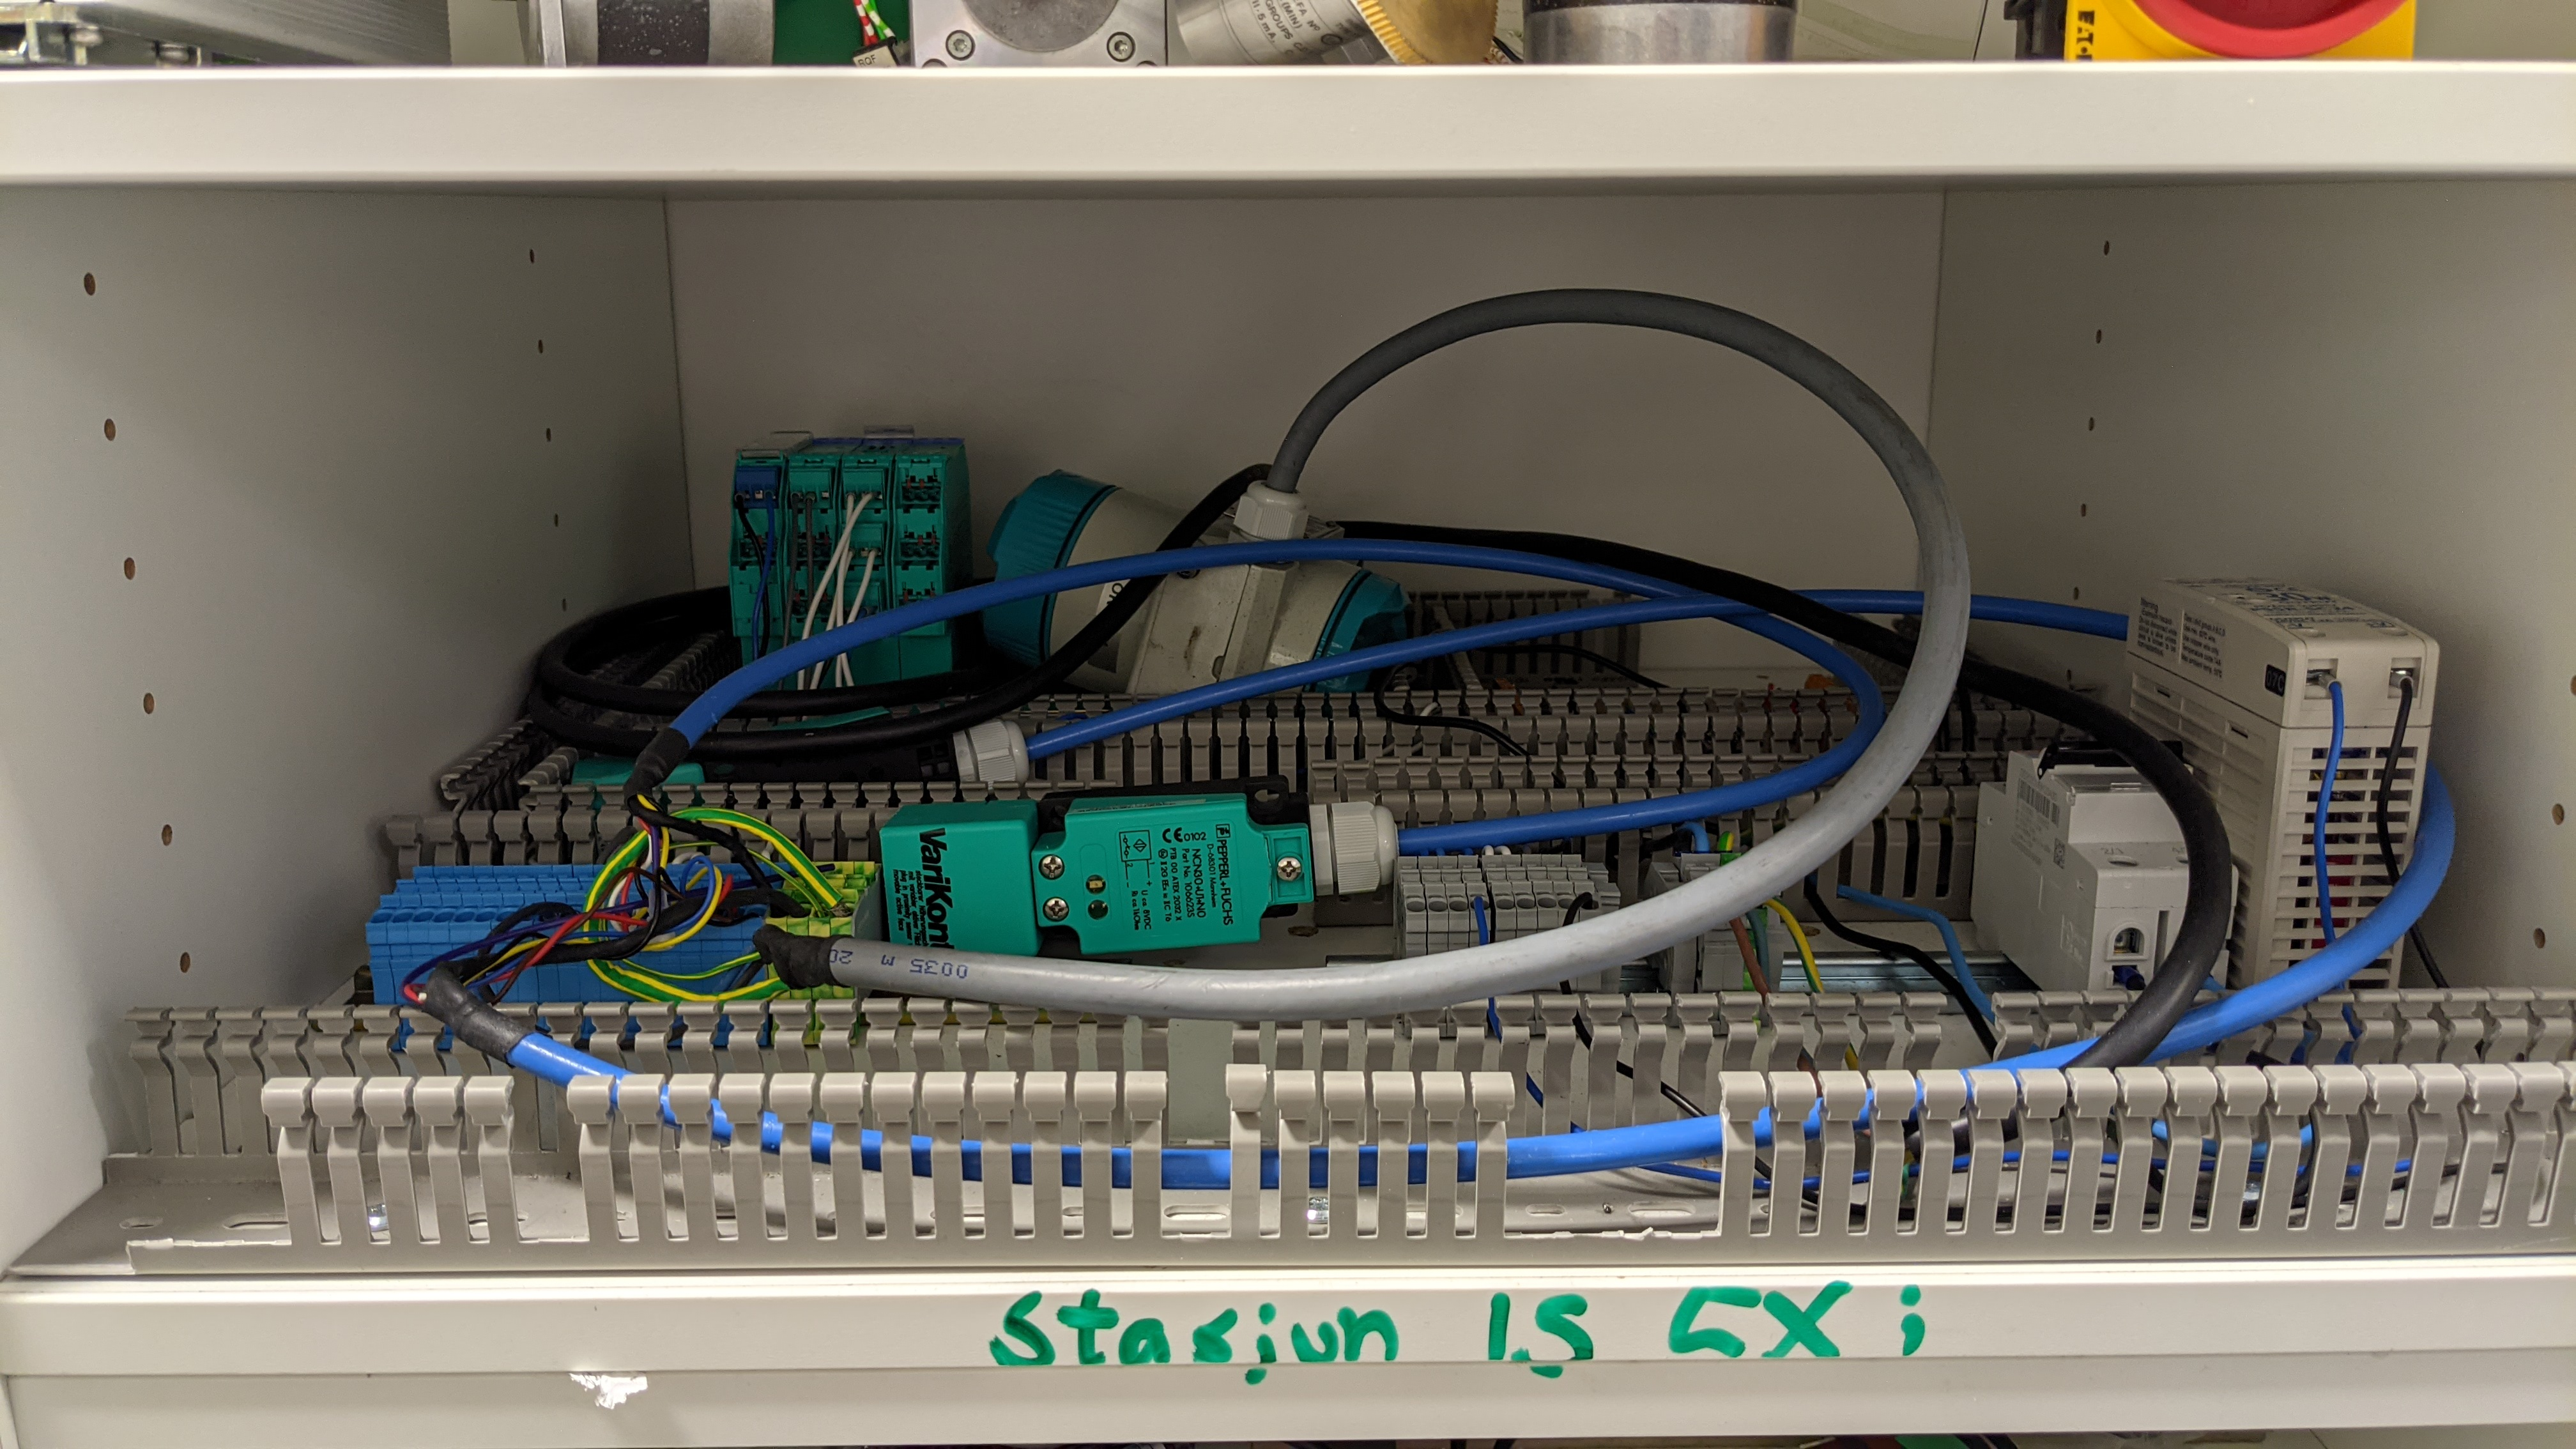
\includegraphics[width=10.5cm]{stasjon15x01.jpg}$$
\textbf{Teorioppgaver}

\vskip 5pt 
Her er noen tekster der du kan lese deg opp på endebrytere

\vskip 5pt 
%\vskip 5pt 
%\href{https://www.edata.omron.com.au/eData/Switches/X019-E1-07.pdf}{Omron komplett katalog}
%\vskip 5pt 
%\href{https://www.ia.omron.com/data_pdf/guide/30/limitswitch_apparatus_tg_e_3_2.pdf}{Omron guide til limit switches}
%\vskip 5pt 
%\href{https://stevenengineering.com/tech_support/PDFs/45LS.pdf}{ukjent}
\vskip 5pt 
\textbf{Teorioppgaver}
\begin{enumerate}
	\item Vis med tegning hva som menes med:
		\begin{itemize}[noitemsep]
			\item Initial posision
			\item pretravel
			\item release point
			\item operation point
			\item Final posistion
			\item Differential
			\item overtravel
		\end{itemize}

	
	\item Hva menes med aktuator?
	\item Hvilke typer aktuator finnes til endebrytere?
	\item Hva menes med switch body?
	\item Forklar forskjellen på plug-inn og ikke plug-in endebryter. 
	\item Hva er forksjllen  på snap action og slow make-break.
	\item Hva menes med positive opening switch.
	\item Hva må en tenke på når en velger på hvilken side av kontaktsettet en setter belastningen på ved to-polt kontaktsett.
	\item Hvilke monteringstyper finnes for endebrytere?
	\item Hva er en Guard Switch?
	\item En kan bruke ulike typer "cam" til å aktuere en endebryter, hvordan velger en rett type?
\end{enumerate}











\end{document}

